%\subsection{Workflow}
\label{sec:workflow}

\begin{figure}
\centering
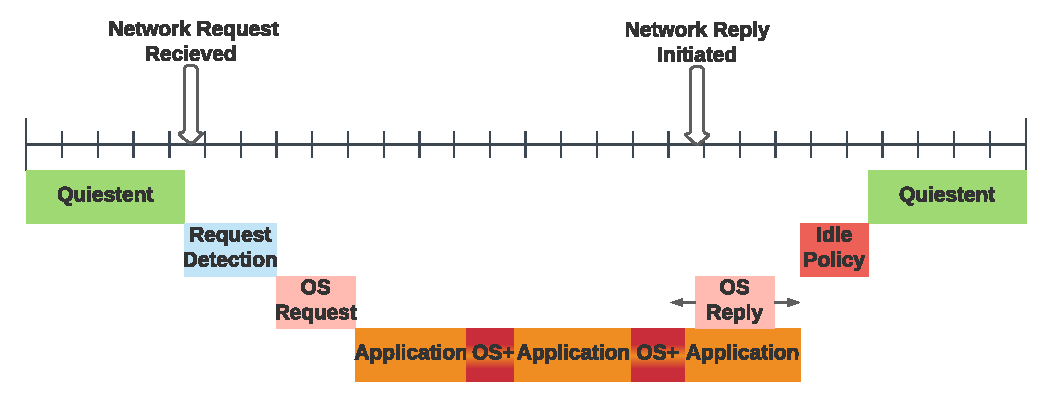
\includegraphics[width=0.5\textwidth]{figures/timeline_chart}
\caption[]{Logical execution timeline for a single application request}
\label{fig:timeline}
\end{figure}

In order to help seed the context of how slowing down processor frequency and ITR-Delay can affect an application's performance and energy, figure~\ref{fig:timeline} presents a generalized breakdown of components along a typical packet receive path. We believe this modeling is applicable across different OS structures and networking hardware's as it details a set of fundamental components that all packet processing frameworks must undergo.

\subsection{Application Perspective}
Figure~\ref{fig:timeline} shows the application is waiting to be woken up to process new packets (a). Next, an interrupt (b) is fired and the OS network stack begins processing the received packet (c). The application level work begins, alongside there are also interspersed OS work which may or may not be in direct support of application(d). The tail end of the application work (e) typically entails a response packet being sent, the period of time with which the response packet is physically sent can proceed in parallel with the rest of the application level work. The end of every request handling (f) also revolves a set of OS policies to decide the next state of the software and hardware. Work is time spent executing instructions required to service a request, it is a function of the software, hardware, and workload itself. Whereas, idle time is a function of arrival rate of packets.

\subsection{Hardware Perspective}
Slowing down of the processor causes an increase in the time spent in portions of application and OS work while reducing energy use. Slowing down of interrupt delays contributes to the increase of time spent in the idle states, the longer a processor idles the more energy it can save.

\subsection{OS Perspective}
OSes overall behaviour is a function of how it behaves during both the working and idle portions of time, there also exists a clear inter-relationship between the two. 

The amount of energy used during this idle period is dependent upon the OS idling policies; in terms of which level of idle state is selected.

\subsection{Equations}

%\subsection{ITR-Delay algorithm}
